%versi 2 (8-10-2016)
\chapter{Landasan Teori}
\label{chap:teori}


\section{Skripsi}
\label{sec:skripsi} 
 
Pada bab ini akan dibahas mengenai dasar teori yang digunakan pada penyusunan tugas akhir. Pembahasan pertama mencakup hal-hal yang berkaitan dengan pengertian kewirausahaan dari umum sampai khusus yaitu kewirausahaan menurut GEM. Pembahasan kedua yaitu tentang CA (Cellular Automata) khususnya tentang ECA (Entrepreneur Cellular Automata). Pembahasan terakhir tentang hal-hal lain yang mendukung implementasi perangkat lunak seperti... 


\section{Arti Kewirausahaan}
\label{sec:artiwirausaha}

\graphicspath{{images/}}

Secara umum arti kewirausahaan merupakan suatu proses dalam mengerjakan sesuatu yang baru dan berbeda yang bermanfaat bagi orang lain atau diri sendiri. Orang yang melakukan proses kewirausahaan adalah wirausaha. Ciri-ciri wirausaha antara lain yaitu berani mengambil risiko, memiliki semangat dan kemauan keras, memiliki jiwa pemimpin, dsb. Tujuan wirausaha sendiri yaitu menciptakan lapangan kerja yang baru dan meningkatkan jumlah para wirausaha di suatu negara.


Kewirausahaan menurut GEM merupakan proses yang terdiri dari fase-fase berbeda mulai dari niat mendirikan suatu usaha, menjalankan suatu usaha baru atau sudah berdiri, sampai dengan penghentian sebuah usaha. Proses ini dimulai dengan keterlibatan individu yang berpotensi untuk menjadi wirausaha, yaitu mereka yang percaya bahwa mereka mempunyai kemampuan untuk memulai suatu usaha, individu yang melihat kesempatan untuk berwirausaha dan individu yang tidak takut gagal dalam memulai suatu usaha.
\begin{figure} 
	\centering  
	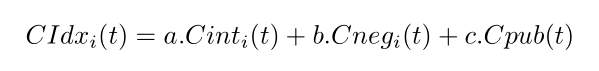
\includegraphics[width=14cm, height=6cm]{Capture}  
	\caption[Gambar Fase Wirausaha]{Gambar Fase Wirausaha} 
	\label{fig:artiwirausaha} 
\end{figure}



 
